\section{Experiments}

\subsection{Model performance on a small size experiment dataset}

\subsubsection{Experimental datasets}

To our knowledge, there's no existing large scale database of annotated X-ray
single particle images categorized by biological/chemical samples.  The Coherent
X-ray Data Bank (CXIDB) serves as ``a permanent public repository of data from
coherent X-ray sources" \cite{maiaCoherentXrayImaging2012}.  We decide to use
the raw data collected in experiment \textit{amo06516}
\cite{liDiffractionDataAerosolized2020}, part of which are also available in
CXIDB (ID 156).  One major difference between raw data and deposited data is
that raw data contain a considerable amount of \textit{non-sample-hit} images,
which are important for real-time hit classification tasks.  For data labeling,
we created a GUI tool (\url{https:
//github.com/carbonscott/hit-labeler}) that allows labeling hits from multiple
 sources, including raw data through \textit{psana}
 \cite{damianiLinacCoherentLight2016} and HDF5 files from CXIDB.  In total, we
 labeled 331 \textit{single-hit}, 170 \textit{multi-hit} and 98
 \textit{non-sample-hit}.  In general, smaller size dataset leads to less data
 variety, which is primarily determined by the aggregation, orientation and
 differaction quality of the biological samples.  Accordingly, we investigate
 the effects of data variety on model performance.  


\subsubsection{Effects of data variety on model performance}

We split our experimental dataset into training set, validation set and test
set.  This is a standard practice that evaluates the goodness of a model on a
given dataset.  Data split can be tricky to handle when the size of a given
dataset is small, which is one of the challenges we will face in training a good
classifier as SPI data are still being collected.  On the other hand, data
augmentation can effortlessly increase the volume of the dataset, but can our
model keep improving its performance with more data augmentation?  The short
answer is `NO', and we think the varieties of uniquely `looking' data would
ultimately impact model performance.  We point out that when a flat detector is
used and aligned perpendicularly to the beam path, any rotation of a diffraction
image along this beam path doesn't add a new variety to the dataset for model
training.  For example, if a training dataset only consists of images generated
by randomly rotating a reference image along the beam path, our model can
successfully identify the labels of those augmented images, but it will likely
fail to recognize images with other unique patterns.  We consider that every
manually labeled image looks uniquely as the chance of labeling two images
differed by a matter of rotation is very little.  In Table \ref{tb : metadata}
and \ref{tb : real performance}, we provide metadata and confusion matrices,
respectively, of four distinct experiments to demonstrate the effects of data
variety on model performance.  

We used the same data partitioning strategy in experiment 1 and 2, which was
25.0\% /37.5\%/73.5\% (train/validate/test) as seen in Table \ref{tb : metadata}
.  We sampled 40 unique images per class, but there were only 18
\textit{non-sample-hit} in the training set.  Then, we applied random rotations
along the beam path to the sampled images, and the total number of images
amounted to 2,000 for the training set and the validation set, respectively.
Here, random rotation was used as a dataset upsampling technique and only
performed after the dataset was partitioned for preventing ``data leakage''
issues \cite{kapoorLeakageReproducibilityCrisis2022}.  In experiment 2, similar
random rotations resulted in 4,000 images in the training set and the validation
set, respectively.  Despite having double the number of images in training,
experiment 2 shows a slightly worse performance, especially in the recall of
predicting \textit{multi-hit} according to Table \ref{tb : real performance}.
Since recall measures the percentage of images correctly predicted for a class,
it implies that the model performance can't be improved through more data
augmentation.  We then examed whether the data variety was too low when only
25.0\% was assigned to the training set, but still wanted to use as few images
as possible.  

We chose a new data partitioning strategy in experiment 3 and 4, which was 50.0\%
/25.0\%/25.0\% (train/validate/test) as depicted in Table \ref{tb : metadata}.
In experiment 3, we still sampled 40 images per class despite having more
candidates to choose thanks to the 50.0\% data split for training.  Again, we
applied similar random rotations to the sampled images, and the total number of
images became 2,000 for training and validation, respectively.  As shown in Table
\ref{tb : real performance}, the model in experiment 3 still can't improve its
recall of 90\% in predicting \textit{multi-hit}.  It seems to signal that 40
images per class is consistently not large enough to cover the data distribution
of the entire dataset.  Then, we decided to sample 80 images per class in
experiment 4, despite only 44 \textit{non-sample-hit} were avaiable in the
training set.  A total of 2,000 images for training and validation, respectively,
were prepared through the same random rotation technique.  In Table \ref{tb :
real performance}, the recall of predicting \textit{multi-hit} in experiment 4
increases to 97\%, a substantial improvement in constrast to $\sim 90\%$ in all
previous three experiments.  Fig. \ref{fig : false single real} gives an
overview of \textit{all} failed \textit{single-hit} cases in experiment 4.

%% Two data spliting
%% strategy are used in the four experiments:  split in experiment 1 and 2; 50.5\%/25.0\%/25.0\% split in
%% experiment 3 and 4.  Obviously, experiment 3 and 4 have larger variety of
%% uniquely `looking' data in the training set.  Experiment 1 and 2 have exactly
%% the same unique images per class, but experiment 2 has a larger data volume as
%% more images are generated by data augmentation.  in Table \ref{tb : performance}, 


\begin{table}

    \caption{
        The metadata of four experiments that are used to illustrate the
        limiting factors of model performance from the training data standpoint.  \#
        denotes `number of images'.  The numbers in the `Unique \# $/$ class' column
        follow the order of \textit{non-sample-hit}, \textit{single-hit} and
        \textit{multi-hit}.  \# (Train) and \# (Validation) are the number of images,
        including those generated from data augmentation, used in model training and
        validation, respectively.  The last column tells the fraction of all
        labeled images used in the training set.  
    }
    \label{tb : metadata}
    %% \renewcommand{\arraystretch}{1.2}

    %% \centering
    %% \resizebox{1.0\textwidth}{!}{
        \begin{tabularx}{\linewdith}{ l c c c c }
            Experiment &   $\dfrac{Unique \#}{class}$  &  \# (Train) & \# (Validation) & $\dfrac{\text{\#Training}}{\text{\#Total}}$ \\
            \hline
            1          &   18;40;40    &  2,000   & 2,000   & 0.25      \\
            2          &   18;40;40    &  4,000   & 4,000   & 0.25      \\
            3          &   40;40;40    &  2,000   & 2,000   & 0.50      \\
            4          &   44;80;80    &  2,000   & 2,000   & 0.50      \\
        \end{tabularx}
    %% }
\end{table}



\begin{table}
    \caption{

        Confusion matrices for all experiments mentioned in Table \ref{tb :
        metadata}.  N, S, M stand for \textit{non-sample-hit},
        \textit{single-hit} and \textit{multi-hit}, respectively.  (A) and (P)
        represent actual label and predicted label, respectively.  Meanwhile,
        ACC, PRE, REC and SPE are acronyms for accuracy, precision, recall and
        specificity, respectively.  

    }

    \label{tb : real performance}
    \begin{tabularx}{\linewidth}{ l | X X X X X X X X }
        \textbf{Experiment 1} &  N(A) & S(A) & M(A) & ACC(\%)  & PRE(\%)  &
        REC(\%)           & SPE(\%)  & F1(\%)   \\
        \hline
        N(P)                  &  335  & 0    & 10   & 99 & 97 & 100          & 98 & 99 \\
        S(P)                  &  0    & 333  & 24   & 97 & \textbf{93} & 99          & 96 & 96 \\
        M(P)                  &  0    & 5    & 293  & 96 & 98 & \textbf{90} & 99 & 94 \\
        \hline
        \textbf{Experiment 2} &       &       &      &      &      &               &      &      \\
        \hline
        N(P)                  &  335  & 1     & 9    & 99 & 97 & 100          & 98 & 99 \\
        S(P)                  &  0    & 327   & 28   & 96 & \textbf{92} & 97          & 97 & 94 \\
        M(P)                  &  0    & 10    & 290  & 95 & 97 & \textbf{89} & 99 & 93 \\
        \hline
        \textbf{Experiment 3} &       &        &      &      &      &               &      &      \\
        \hline
        N(P)                  &  331  & 0      & 13   & 99 & 96 & 100          & 98 & 98 \\
        S(P)                  &  0    & 339    & 19   & 97 & \textbf{95} & 98          & 97 & 96 \\
        M(P)                  &  0    & 6      & 292  & 96 & 98 & \textbf{90} & 99 & 94 \\
        \hline
        \textbf{Experiment 4} &       &        &      &      &      &               &      &      \\
        \hline
        N(P)                  &  331  & 1      & 7    & 99 & 98 & 100          & 99 & 99 \\
        S(P)                  &  0    & 340    & 4    & 99 & \textbf{99} & 99          & 99 & 99 \\
        M(P)                  &  0    & 4      & 313  & 98 & 99 & \textbf{97} & 99 & 98 \\
    \end{tabularx}

\end{table}


\begin{figure}
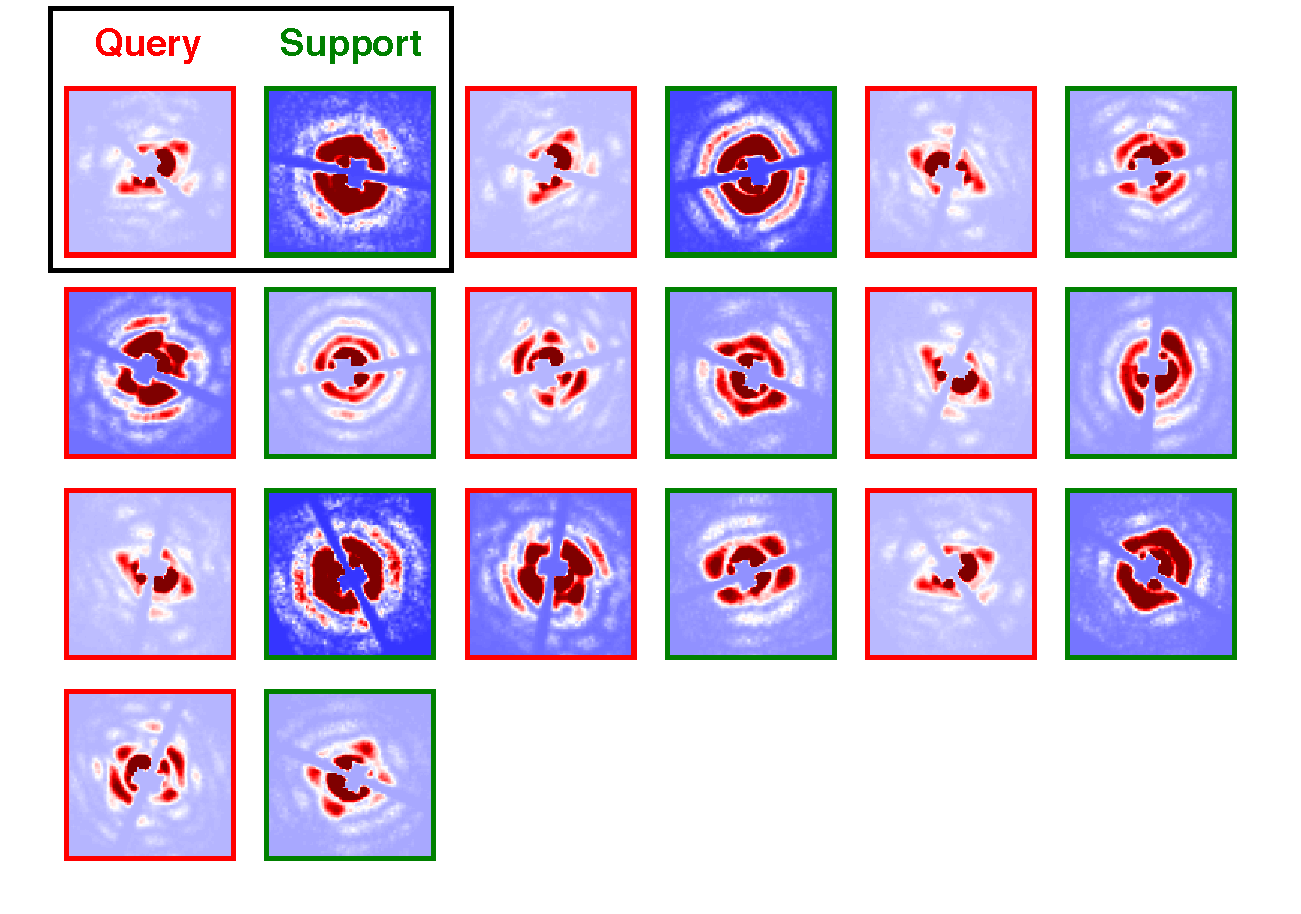
\includegraphics[width=\textwidth,keepaspectratio]
{figures/false_label.single.real.pdf}

\caption{\textit{All} falsely labeled \textit{single-hit} in experiment 4.
Queried images are put into red boxes, whereas the corresponding `most similar'
supported images chosen by our model are enclosed in green boxes.}

\label{fig : false single real}
\end{figure}


To sum it up, data variety plays a critical role in dictating the model
performance that requires covering enough data space.  From a practical
perspective, a good precision of predicting \textit{single-hit} would suffice
for our use.  However, it is recall that unveils whether the data variety is
sufficient, which is the underlying limiting factor that prevents the model from
achieving a better precision.  Additionally, we can label far fewer images for
model training if a higher error rate is acceptable by the downstream particle
reconstruction process.  


\subsubsection{Effects of dead detector areas on model performance}

It's not uncommon to encounter a detector with dead pixel areas during a SPI
experiment.  We trained our model on SPI images artificially occluded by a mask
half of the size of an image.  We reused the experiment dataset mentioned
before.  More specifically, We employed 50\% data for model training and 25\%
data each for validation and testing, respectively.  Apart from image occlusion,
the same data preprocessing procedures used in experiment 2 were also applied,
including image cropping, in-plane random rotation, and downsampling.  Through
the random in-plane rotation, we prepared 4,000 images for model training.  Our
model achieves an impressive 100\% (after rounding) precision in predicting
\textit{single-hit}, as seen in Table \ref{tb : real performance mask}, even
with half of its diffraction pattern occluded.  Fig. \ref{fig : true single
real} shows a collection of queried hits correctly labeled according to their
`most similar' support hits.  Overall, this result demonstrates that our model
can still have good classification performance in the presence of dead pixel
areas on a detector.  

\begin{table}
    \caption{

        Confusion matrix for the experiment investigating data occlusion on
        model performance.  The acronyms used in this table are consistent with
        the definitions specified in Table \ref{tb : real performance}.

    }

    \label{tb : real performance mask}

        \begin{tabularx}{\linewidth}{ l | X X X X X X X X }
                                  &  N(A) & S(A) & M(A) & ACC(\%)  & PRE(\%)  &
                                  REC(\%)           & SPE(\%)  & F1(\%)   \\
            \hline
            N(P)                  &  331  & 0    &  5   & 99 & 99 & 100 & 99 & 99 \\
            S(P)                  &  0    & 340  &  1   & 99 & \textbf{100} & 99 & 1.00 & 99 \\
            M(P)                  &  0    & 5    & 318  & 99 & 98 & 98 & 99 & 98 \\
        \end{tabularx}
    %% }
\end{table}


\begin{figure}
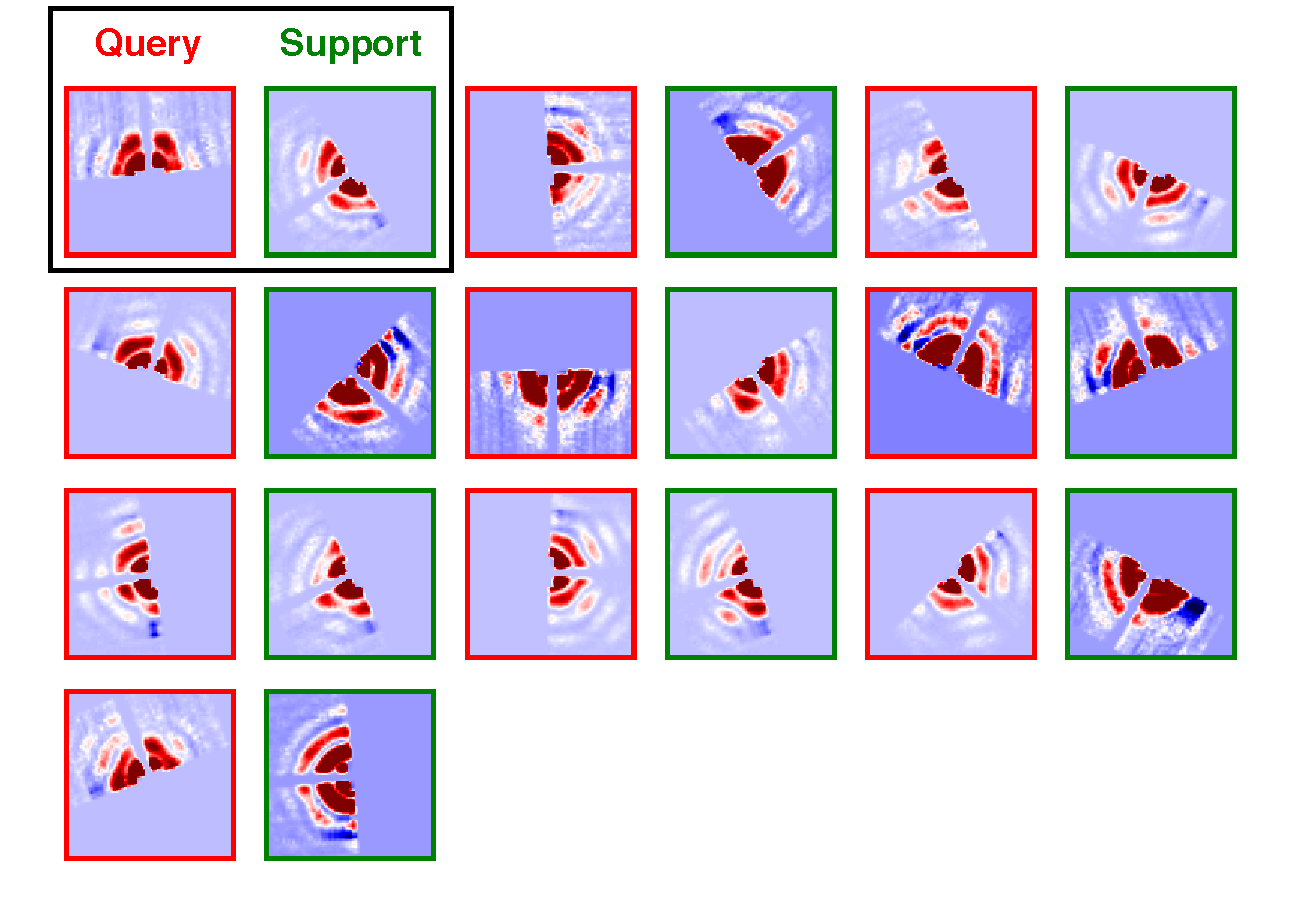
\includegraphics[width=\textwidth,keepaspectratio]
{./figures/true_label.single.real.pdf}

\caption{A partial collection of correctly labeled \textit{single-hit} in the
experiment where SPI hits are artificially occluded to mimic the behavior of a
detector with dead pixel areas.  Queried images are put into red boxes, whereas
the corresponding `most similar' supported images chosen by our model are
enclosed in green boxes.}

\label{fig : true single real}
\end{figure}


\subsection{Model generalizability assessed using simulated hits}

According to the FaceNet paper \cite{schroffFaceNetUnifiedEmbedding2015}, a CNN
vision core trained through triplet loss function can identify faces of nearly 8
million identities.  It has intrigued us whether our CNN vision core that is
trained in a similar manner can recognize SPI hits (like human faces) resulted
from various PDB entries (like human identities).  If the
\textit{one-model-fits-all} scenario is true, it will profoundly impact how hit
classification can possibly be done in real experiments.  


\subsubsection{Simulated datasets}

There's no existing large scale database of annotated SPI images generated by
physics-based simulation.  We resorted to \textit{skopi}
\cite{peckSkopiSimulationPackage2022}, a GPU-based program for simulating
diffractive images from noncrystalline biomolecules, for concurrently simulating
high-resolution SPI scattering patterns and providing accurate labels in an
automated manner at scale.  Considering most biological samples in the past SPI
techniques are large virus particles, we are interested in training our hit
classifier on \textit{large} single particles.  PDB statistics offers direct
insights into PDB data distribution by molecular weight (\url{https:
//www.rcsb.org/stats/distribution-molecular-weight-structure}).  Accordingly, we
focus on those particles with molecular weights over 380 $KDa$.  Fig.  \ref{fig:
num atom per bio assem} describes the population frequency of the atom number
per biological assembly with each area representing 50 PDB items.  The atom
numbers spread across three orders of magnitudes ($10^4\text{-}10^6$).  96.0\%
of \textit{large} particles have $10^4$ atoms, and only 1.2\% have massive
$10^6$ atom numbers. Simulated datasets are generated by setting the detector
distance at 100.0 $mm$ and photon energy at 1.660 $keV$.  In total, we simulated
0.5 million SPI hits from 5,778 PDB entries, and the type of hit ranges from
\textit{single-hit} to \textit{quadruple-hit}.  There's no example of
\textit{non-sample-hit} in the simulated dataset.

We divided PDB entries into a training group and a testing group.  Our model had
access to the hits simulated only from the training group during model training
and validation.  Then, the trained model were tested against the hits
simulated only from the PDBs in the testing group.  We chose three ways to
divide PDBs , which were 10\%/90\%, 50\%/50\% and 80\%/20\% (\%training/\%testing).  
The common PDBs in the three testing groups contributed to hits for the
ultimate testing, which contained 115,200 hits from 1,154 PDBs.  

\begin{figure}
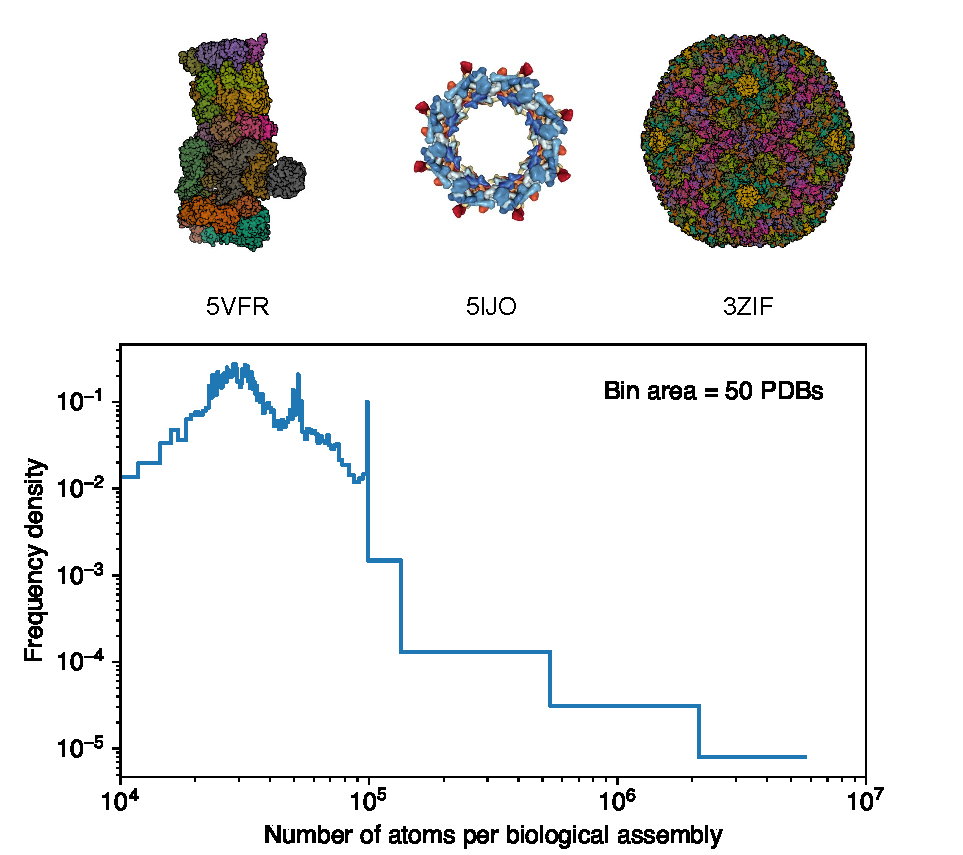
\includegraphics[width=1.0\textwidth,keepaspectratio]
{./figures/num_atom_per_bio_assem.pdf}

\caption{Number of atoms per biological assembly.  Molecular images are taken
from Structure Summary pages from RCSB PDB(rcsb.org) of PDB ID
5VFR\cite{zhuStructuralMechanismNucleotidedriven2018}, 5IJO\cite{kosinskiMolecularArchitectureInner2016} and
3ZIF\cite{chengCryoEMStructuresTwo2014}.}

\label{fig: num atom per bio assem}
\end{figure}


\subsubsection{Performance}

Our model achieved a test accuracy from 90.06\% to 93.38\% on SPI hits with no
noise applied to, which were originally simulated from a diverse collection of
PDB entries.  We investigated four factors that might impact the model
performances.  The primary factor was the noise applied to SPI hits.  In
experiment A1 and A2 in Table \ref{tb : simulated performance}, we kept hits
unperturbed in A1, but applied Poisson noise to hits in A2 followed by Gaussian
noise at the standard deviation of 0.15.  We trained our model using 200K
training examples/hits collected from 80\% PDBs.  The margin in the triplet loss
function was set to be 0.2.  Then, we used 100K hits in the other 20\% PDBs for
testing the model generalizability.  The model in experiment A1 demonstrated an
accuracy of 93.38\%, whereas the noisy hits in A2 rendered the model accuracy
down to 86.94\%, a 6.44\% decline.  The other three factors, which were \%PDB
for training, sample size and triplet loss margin, played a secondary role in
dictating the model performance.  Nonetheless, an astonishing finding in
experiment B3, C3 and D3 was that our model kept up its accuracy above 90\% even
when trained on hits from only 10\% of PDBs.  Lastly, sample size and triplet
loss margin only turned out to have diminishing effects on improving model
performance.  Fig.  \ref{fig : false single simulated} is an overview of
\textit{all} failed \textit{single-hit} cases in experiment A2.


\begin{table}
    \caption{Experiments that demonstrate the model performances in various
    conditions.}
    \label{tb : simulated performance}
    \begin{tabularx}{\linewidth}{ l | X X X X X }
        Experiment  &
        PDB$_{\text{train}}$ (\%) &
        Sample Size &
        Margin,$\alpha$ &
        Accuracy (\%) \\
        \hline
        A1  & 80 & 200K &  0.2 & 93.38 \\
        A2 (noise)  & 80 & 200K &  0.2 & 86.94 \\
        \hline
        B1  & 80 & 100K &  0.2 & 93.23 \\
        B2  & 50 & 100K &  0.2 & 92.91 \\
        B3  & 10 & 100K &  0.2 & 90.86 \\
        \hline
        C1  & 80 & 100K &  2.0 & 91.56 \\
        C2  & 50 & 100K &  2.0 & 91.00 \\
        C3  & 10 & 100K &  2.0 & 90.84 \\
        \hline
        D1  & 80 & 40K  &  2.0 & 90.20 \\
        D2  & 50 & 40K  &  2.0 & 90.69 \\
        D3  & 10 & 40K  &  2.0 & 90.06 \\
    \end{tabularx}
\end{table}


% Insert the figure HERE and TOP..
\begin{figure}
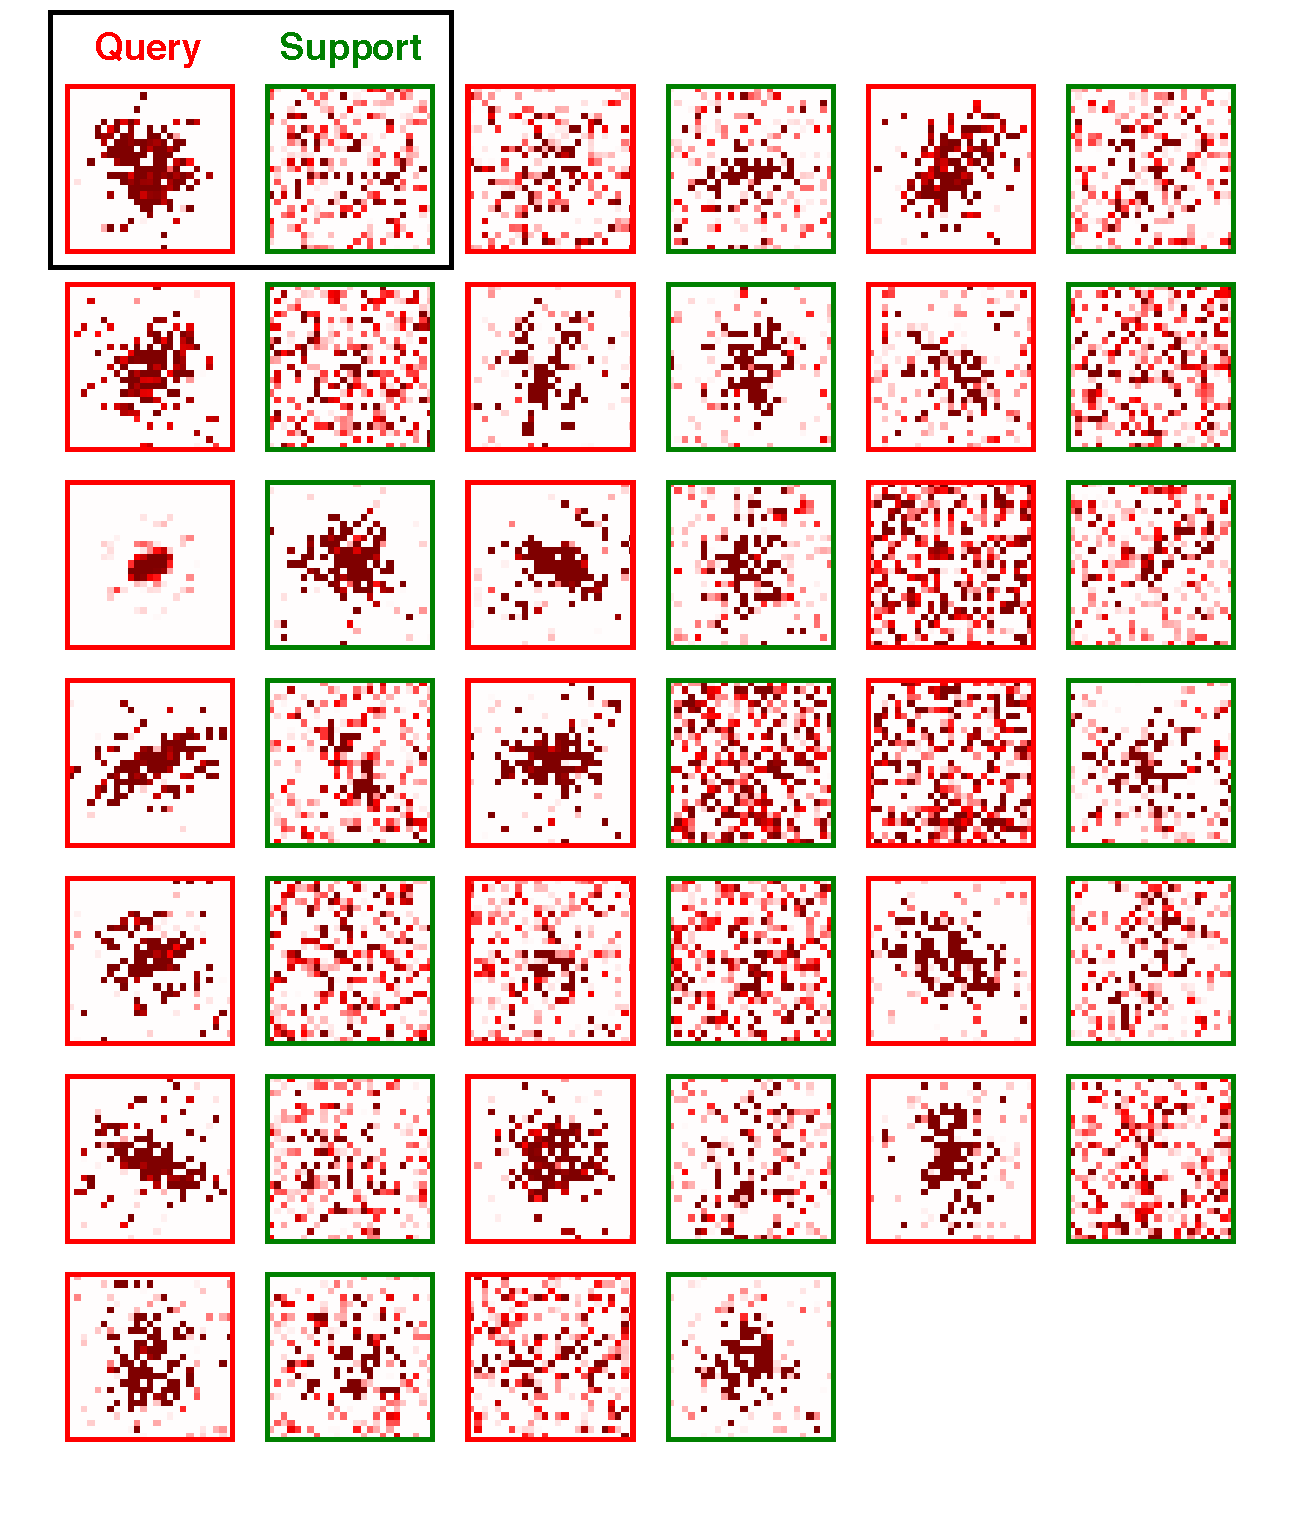
\includegraphics[width=\textwidth,height=0.8\textheight,keepaspectratio]
{figures/false_label.single.simulated.pdf}

\caption{A partial collection of falsely labeled \textit{single-hit} in our test
simulated dataset.  Query images are put into red boxes, whereas the
corresponding `most similar' supported images chosen by our model are enclosed
in green boxes.  The negative intensities are artificially reset to zero for
cleaner visual purposes.  }

\label{fig : false single simulated}
\end{figure}


\subsection{Revisit the model performance observed in experimental dataset,
but with a larger dataset using simulation}

We've seen great performance of our model on an experimental dataset comprising
about 600 manually labeled SPI hits.  More specifically, our model reached a
99\% precision in predicting \textit{single-hit} by training on only 80
\textit{single-hit}, 80 \textit{multi-hit} and 44 \textit{non-sample-hit}.
However, can our model perform consistently on a larger dataset while using
the same number of training examples?  Complicated by the scarcity of labeled
experimental datasets, we once again turned to simulating 2,000
\textit{single-hit}, 500 \textit{double-hit}, 300 \textit{triplet-hit} and 200
\textit{quadruple-hit} on an artifical pnCCD detector with \textit{skopi}.
Similar to the simulated dataset used in the generalizability study, there's no
\textit{non-sample-hit} class, but we considered everything other than
\textit{single-hit} as \textit{multi-hit}.  

We set aside 50\% of the simulated hits for training but only limit to 80 hits
per class visible to our model.  The rest of the dataset were equally divided by
the validation set and the test set.  Afterwards, data preprocessing was applied
in the same manner, which encompassed applying Possion noise and Gaussian noise,
ROI cropping, random in-plane rotation and downsampling.  In Table \ref{tb :
simulated performance large}, the confusion matrix directly indicates that the
model delivers an execellent classification performance on a larger 
dataset.  Therefore, we can optimistically conclude that our model can have a
consistently good performance whilst trained on a small size training set.  

\begin{table}
    \caption{

        Confusion matrix for the experiment investigating model performance on
        a larger dataset.  The acronyms used in this table are consistent with
        the definitions specified in Table \ref{tb : real performance}.

    }

    \label{tb : simulated performance large}

        \begin{tabularx}{\linewidth}{ l | X X X X X X X }
                                  &   S(A) & M(A) & ACC(\%)  & PRE(\%)  & REC(\%)
                                  & SPE(\%)  & F1(\%)   \\
            \hline
            S(P)                  &   477  &  5   & 99 & 99 & 100 & 99 & 99 \\
            M(P)                  &   1    & 517  & 99 & 100 & 99 & 100 & 99 \\
        \end{tabularx}
    %% }
\end{table}


%% Table \ref{tb: SPI
%% experiments} is a list of all SPI experiments documented on CXIDB.  
%% \begin{table}
%%     \caption{All SPI experiments documented on CXIDB.}
%%     \label{tb: SPI experiments}
%%     %% \renewcommand{\arraystretch}{1.2}
%%     %% \resizebox{1.0\textwidth}{!}{
%%         \begin{tabularx}{\textwidth}{ l l X }
%%             CXIDB ID & Light Source & Sample \\
%%             \hline
%%             1        & LCLS         & Mimivirus                                                       \\
%%             2        & LCLS         & Mimivirus                                                       \\
%%             3        & FLASH        & FIB etched 20-nm-thick silicon nitride membrane                 \\
%%             4-8      & ALS          & Gold labeled frozen dried Saccharomyces cerevisiae yeast cells  \\
%%             9        & FLASH        & Iron Oxide Ellipsoids                                           \\
%%             10       & LCLS         & Nanorice                                                        \\
%%             11       & LCLS         & Magnetosomes                                                    \\
%%             12       & LCLS         & Tobacco mosaic virus                                            \\
%%             13       & LCLS         & T4 bacteriophage                                                \\
%%             14       & LCLS         & Paramecium bursaria Chlorella virus                             \\
%%             19       & LCLS         & Airborne Particulate Matter (Soot)                              \\
%%             20       & LCLS         & Clusters of Polystyrene Spheres                                 \\
%%             25       & LCLS         & Carboxysomes                                                    \\
%%             26       & LCLS         & Cyanobium gracile                                               \\
%%             27       & LCLS         & Synechococcus elongatus                                         \\
%%             28       & ALS          & 50 nm colloidal gold particles                                  \\
%%             30       & LCLS         & Mimivirus                                                       \\
%%             36       & LCLS         & Rice Dwarf Virus                                                \\
%%             37       & LCLS         & Cyanobium gracile and Synechococcus elongtatus                  \\
%%             56       & LCLS         & Omono River Virus                                               \\
%%             57       & LCLS         & Gold core and palladium shell nanoparticles                     \\
%%             58       & LCLS         & Coliphage PR772                                                 \\
%%             78       & LCLS         & RNA polymerase II                                               \\
%%             84       & ESRF         & Gold structure (largest diameter about 1.1 um)                  \\
%%             88       & LCLS         & PR772                                                           \\
%%             119      & LCLS         & Sucrose                                                         \\
%%             146      & FLASH        & Xenon nanoclusters                                              \\
%%             155      & LCLS         & Melbournevirus                                                  \\
%%             156      & LCLS         & Coliphage PR772                                                 \\
%%         \end{tabularx}
%%     %% }
%% \end{table}
